% Section and subsections will appear in the presentation overview
% and table of contents.
\section{Introducción}

\subsection{Motivación}

\begin{frame}{Introducción}{Motivación}
  \begin{itemize}
  \item {
    Estudios de sistemas con múltiples componenentes.
  }
  \item {
    Reducción del costo computacional.
  }
  \end{itemize}
  
  %~ \begin{figure}[ht]
  %~ \centering{}\includegraphics[scale = 0.35]{cold-source-mot.png}
  %~ \caption
  %~ {Esquema del circuito de deuterio en una fuente fría de neutrones.}
  %~ \label{ffmotivacion}
  %~ \end{figure}
  
  %~ \fboxsep=0pt
  %~ \noindent\fbox{%
  %~ \begin{minipage}[t]{0.3\linewidth}
      %~ \centering
      %~ \includegraphics[scale=0.25]{cold-source-mot.png}
      %~ \caption[]{Esquema del circuito de deuterio en una fuente fría de neutrones.}
      %~ \label{fuente-fria-mot}
  %~ \end{minipage}}%
  %~ \hfill%
  %~ \fbox{%
  %~ \begin{minipage}[t]{0.65\linewidth}
      %~ \centering
      %~ \includegraphics[scale=0.2]{ssp-mot.png}
      %~ \caption[]{t=250 s}
      %~ \label{ssp-mot}	
  %~ \end{minipage}
  %~ }

  \begin{figure}[ht]
    \begin{minipage}{0.4\linewidth}
      \centering
      %\includegraphics[scale=0.3]{cold-source-mot.png}
      \includegraphics[scale=0.17]{deuterio.png}
      \caption[]{Esquema del circuito de deuterio en una fuente fría de neutrones.}
      \label{fuente-fria-mot}	
    \end{minipage}
    \begin{minipage}{0.58\linewidth}
      \centering
      \includegraphics[scale=0.19]{ssp-mot.png}
      \caption[]{Esquema del Segundo Sistema de Parada del reactor RA-10.}
      \label{ssp-mot}	
    \end{minipage}
    %\caption[]{}  
    \label{aasdasd}
  \end{figure}
  
\end{frame}

\subsection{Abordaje del modelado}
\begin{frame}{Introducción}{Abordaje del modelado}

  \begin{figure}[ht]
%~ 
    \begin{minipage}{0.58\linewidth}
      \begin{itemize}
      \item <2-> Desglosar en subsistemas
      \item <3-> Identificar uniones que relacionan interfaces de acoplamiento
      \item <4-> Identificar pares de variables incógnitas en cada interfaz
      \item <5-> Total de incógnitas: 2N
        \begin{itemize}
        \item <6-> N ecuaciones de continuidad que relacionan las incógnitas entre dos interfaces contiguas de distintos subsistemas
        \item <7-> N ecuaciones modelos (acopladas) que relacionan las incógnitas (según selección de condiciones de borde)
        %\item <7-> N ecuaciones modelos que relacionan las incógnitas de la misma interfaz de cada subsistema
        \end{itemize} 
      \item <8-> Seleccionar método numérico y resolver con acoplamiento fuerte
      \end{itemize}    
    \end{minipage}
%~ 
    \begin{minipage}{0.4\linewidth}
      \centering
      \includegraphics[scale=0.2]{coupling_systems.png}
      %\caption[]{Análisis de un sistema mediante el Método de Descomposición Disjunta de Dominios.}
      \label{esquma-DDM}
    \end{minipage}
        %~ 
    %\caption[]{}  
    \label{aasdasd}
  \end{figure}
  
  
\end{frame}



% You can reveal the parts of a slide one at a time
% with the \pause command:
\begin{frame}{Introducción}{Abordaje del modelado: Ejemplo}
Ejemplo: El dominio $\Omega$ representa una barra de largo $L$, coficiente de conductividad térmica $k$ y fuente interna de energía $f$.
Calcular el campo de temperaturas en $\Omega$ mediante el método
de Descomposición Disjunta de Dominios. Modelo:
\begin{equation*}
\left\{\begin{matrix}
-k \Delta u=f \\
\left.u\right|_{\partial\Omega}=0
\end{matrix}\right.
\label{ecuacion-calor}
\end{equation*}

\centering
%\raggedleft
  \begin{tikzpicture}[scale=0.750]
	\node at (12.5,4em) (om) {$\Omega$};

	\node at (7.5,5.9em) (Olabel) {0}; % 0
	\node at (7.5,5em) (O) {}; % point 0

	\node at (14.5,6.9em) (clabel) {c}; % c
	\node at (14.5,5em) (c) {}; % point c

	\node at (17.5,5.9em) (llabel) {L}; % L
	\node at (17.5,5em) (l) {}; % point L

	\draw[line width=1pt, o-|] (O) -- (c.center); % primer extremo de barra completa
	\draw[line width=1pt, |-o] (c.center) -- (l); % segundo extremo de barra completa
%~ 
	%~ \draw[line width=0.8pt,->] (11,3.5em) -- (10,1.5em); % primer flecha
	%~ \draw[line width=0.8pt,->] (16,3.5em) -- (17,1.5em); % segunda flecha
%~ 
	%~ \node at (10,-1em) (om1) {$\Omega_1$};
	%~ \node at (6.5,0.9em) (O1label) {0};
	%~ \node at (6.5,0em) (O1) {};
	%~ \node at (13.5,0.9em) (c1label) {c};
	%~ \node at (13.5,0em) (c1) {};
%~ 
	%~ \draw[line width=1pt, o-o] (O1) -- (c1); % primer barra
%~ 
	%~ \node at (17,-1em) (om2) {$\Omega_2$};
	%~ \node at (15.5,0.9em) (c2label) {c};
	%~ \node at (15.5,0em) (c2) {};
	%~ \node at (18.5,0.9em) (l2label) {L};
	%~ \node at (18.5,0em) (l2) {};
%~ 
	%~ \draw[line width=1pt, o-o] (c2) -- (l2); % segunda barra
  \end{tikzpicture}

\end{frame}


% You can reveal the parts of a slide one at a time
% with the \pause command:
\begin{frame}{Introducción}{Abordaje del modelado: Ejemplo}

\begin{itemize}
\item 1. Descomponer el dominio
\end{itemize}

\centering
%\raggedleft
  \begin{tikzpicture}[scale=0.750]
	\node at (12.5,4em) (om) {$\Omega$};

	\node at (7.5,5.9em) (Olabel) {0}; % 0
	\node at (7.5,5em) (O) {}; % point 0

	\node at (14.5,6.9em) (clabel) {c}; % c
	\node at (14.5,5em) (c) {}; % point c

	\node at (17.5,5.9em) (llabel) {L}; % L
	\node at (17.5,5em) (l) {}; % point L

	\draw[line width=1pt, o-|] (O) -- (c.center); % primer extremo de barra completa
	\draw[line width=1pt, |-o] (c.center) -- (l); % segundo extremo de barra completa

	\draw[line width=0.8pt,->] (11,3.5em) -- (10,1.5em); % primer flecha
	\draw[line width=0.8pt,->] (16,3.5em) -- (17,1.5em); % segunda flecha

	\node at (10,-1em) (om1) {$\Omega_1$};
	\node at (6.5,0.9em) (O1label) {0};
	\node at (6.5,0em) (O1) {};
	%~ \node at (13.5,0.9em) (c1label) {c};
	\node at (13.5,0em) (c1) {};

	\draw[line width=1pt, o-] (O1) -- (c1); % primer barra

	\node at (17,-1em) (om2) {$\Omega_2$};
	%~ \node at (15.5,0.9em) (c2label) {c};
	\node at (15.5,0em) (c2) {};
	\node at (18.5,0.9em) (l2label) {L};
	\node at (18.5,0em) (l2) {};

	\draw[line width=1pt, -o] (c2) -- (l2); % segunda barra
  \end{tikzpicture}

\end{frame}

% You can reveal the parts of a slide one at a time
% with the \pause command:
\begin{frame}{Introducción}{Abordaje del modelado: Ejemplo}

\begin{itemize}
\item 1. Descomponer el dominio
\item 2. Reconocer interfaces de acople
\end{itemize}

\centering
%\raggedleft
  \begin{tikzpicture}[scale=0.750]
	\node at (12.5,4em) (om) {$\Omega$};

	\node at (7.5,5.9em) (Olabel) {0}; % 0
	\node at (7.5,5em) (O) {}; % point 0

	\node at (14.5,6.9em) (clabel) {c}; % c
	\node at (14.5,5em) (c) {}; % point c

	\node at (17.5,5.9em) (llabel) {L}; % L
	\node at (17.5,5em) (l) {}; % point L

	\draw[line width=1pt, o-|] (O) -- (c.center); % primer extremo de barra completa
	\draw[line width=1pt, |-o] (c.center) -- (l); % segundo extremo de barra completa

	\draw[line width=0.8pt,->] (11,3.5em) -- (10,1.5em); % primer flecha
	\draw[line width=0.8pt,->] (16,3.5em) -- (17,1.5em); % segunda flecha

	\node at (10,-1em) (om1) {$\Omega_1$};
	\node at (6.5,0.9em) (O1label) {0};
	\node at (6.5,0em) (O1) {};
	\node at (13.5,0.9em) (c1label) {c};
	\node at (13.5,0em) (c1) {};

	\draw[line width=1pt, o-o] (O1) -- (c1); % primer barra

	\node at (17,-1em) (om2) {$\Omega_2$};
	\node at (15.5,0.9em) (c2label) {c};
	\node at (15.5,0em) (c2) {};
	\node at (18.5,0.9em) (l2label) {L};
	\node at (18.5,0em) (l2) {};

	\draw[line width=1pt, o-o] (c2) -- (l2); % segunda barra
  \end{tikzpicture}

\end{frame}

% You can reveal the parts of a slide one at a time
% with the \pause command:
\begin{frame}{Introducción}{Abordaje del modelado: Ejemplo}

\begin{itemize}
\item 1. Descomponer el dominio
\item 2. Reconocer interfaces de acople
\item 3. Identificar pares de variables de acoplamiento
\end{itemize}

\centering
%\raggedleft
  \begin{tikzpicture}[scale=0.750]%, every node/.style={scale=0.75}]
	\node at (12.5,4em) (om) {$\Omega$};

	\node at (7.5,5.9em) (Olabel) {0}; % 0
	\node at (7.5,5em) (O) {}; % point 0

	\node at (14.5,6.9em) (clabel) {c}; % c
	\node at (14.5,5em) (c) {}; % point c

	\node at (17.5,5.9em) (llabel) {L}; % L
	\node at (17.5,5em) (l) {}; % point L

	\draw[line width=1pt, o-|] (O) -- (c.center); % primer extremo de barra completa
	\draw[line width=1pt, |-o] (c.center) -- (l); % segundo extremo de barra completa

	\draw[line width=0.8pt,->] (11,3.5em) -- (10,1.5em); % primer flecha
	\draw[line width=0.8pt,->] (16,3.5em) -- (17,1.5em); % segunda flecha

	\node at (10,-1em) (om1) {$\Omega_1$};
	\node at (6.5,0.9em) (O1label) {0};
	\node at (6.5,0em) (O1) {};
	\node at (13.5,0.9em) (c1label) {c};
	\node at (13.2,-1.7em) (c1label) {\scriptsize $\{T_{S_1}, q''_{S_1}\}$};
	\node at (13.5,0em) (c1) {};

	\draw[line width=1pt, o-o] (O1) -- (c1); % primer barra

	\node at (17,-1em) (om2) {$\Omega_2$};
	\node at (15.5,0.9em) (c2label) {c};
  \node[align=center] at (15.7,-1.7em) (c1label) {\scriptsize $\{T_{S_2}, q''_{S_2}\}$};
	\node at (15.5,0em) (c2) {};
	\node at (18.5,0.9em) (l2label) {L};
	\node at (18.5,0em) (l2) {};

	\draw[line width=1pt, o-o] (c2) -- (l2); % segunda barra
  \end{tikzpicture}

\end{frame}

% You can reveal the parts of a slide one at a time
% with the \pause command:
\begin{frame}{Introducción}{Abordaje del modelado: Ejemplo}

%\centering
\raggedleft
  \begin{tikzpicture}[scale=0.50, every node/.style={scale=0.7}]
	\node at (12.5,4em) (om) {$\Omega$};

	\node at (7.5,5.9em) (Olabel) {0}; % 0
	\node at (7.5,5em) (O) {}; % point 0

	\node at (14.5,6.9em) (clabel) {c}; % c
	\node at (14.5,5em) (c) {}; % point c

	\node at (17.5,5.9em) (llabel) {L}; % L
	\node at (17.5,5em) (l) {}; % point L

	\draw[line width=1pt, o-|] (O) -- (c.center); % primer extremo de barra completa
	\draw[line width=1pt, |-o] (c.center) -- (l); % segundo extremo de barra completa

	\draw[line width=0.8pt,->] (11,3.5em) -- (10,1.5em); % primer flecha
	\draw[line width=0.8pt,->] (16,3.5em) -- (17,1.5em); % segunda flecha

	\node at (10,-1em) (om1) {$\Omega_1$};
	\node at (6.5,0.9em) (O1label) {0};
	\node at (6.5,0em) (O1) {};
	\node at (13.5,0.9em) (c1label) {c};
	\node at (13.2,-1.7em) (c1label) {\scriptsize $\{T_{S_1}, q''_{S_1}\}$};
	\node at (13.5,0em) (c1) {};

	\draw[line width=1pt, o-o] (O1) -- (c1); % primer barra

	\node at (17,-1em) (om2) {$\Omega_2$};
	\node at (15.5,0.9em) (c2label) {c};
  \node[align=center] at (15.7,-1.7em) (c1label) {\scriptsize $\{T_{S_2}, q''_{S_2}\}$};
	\node at (15.5,0em) (c2) {};
	\node at (18.5,0.9em) (l2label) {L};
	\node at (18.5,0em) (l2) {};

	\draw[line width=1pt, o-o] (c2) -- (l2); % segunda barra
  \end{tikzpicture}

\begin{itemize}
\item 4. Ecuaciones de continuidad: 
\begin{equation*}
\left\{\begin{matrix}
T_{S_1} = T_{S_2}=T \\
q''_{S_1} = q''_{S_2}=q''
\end{matrix}\right.
\end{equation*}
\end{itemize}

\end{frame}


% You can reveal the parts of a slide one at a time
% with the \pause command:
\begin{frame}{Introducción}{Abordaje del modelado: Ejemplo}

%\centering
\raggedleft
  \begin{tikzpicture}[scale=0.50, every node/.style={scale=0.7}]
	\node at (12.5,4em) (om) {$\Omega$};

	\node at (7.5,5.9em) (Olabel) {0}; % 0
	\node at (7.5,5em) (O) {}; % point 0

	\node at (14.5,6.9em) (clabel) {c}; % c
	\node at (14.5,5em) (c) {}; % point c

	\node at (17.5,5.9em) (llabel) {L}; % L
	\node at (17.5,5em) (l) {}; % point L

	\draw[line width=1pt, o-|] (O) -- (c.center); % primer extremo de barra completa
	\draw[line width=1pt, |-o] (c.center) -- (l); % segundo extremo de barra completa

	\draw[line width=0.8pt,->] (11,3.5em) -- (10,1.5em); % primer flecha
	\draw[line width=0.8pt,->] (16,3.5em) -- (17,1.5em); % segunda flecha

	\node at (10,-1em) (om1) {$\Omega_1$};
	\node at (6.5,0.9em) (O1label) {0};
	\node at (6.5,0em) (O1) {};
	\node at (13.5,0.9em) (c1label) {c};
	\node at (13.2,-1.7em) (c1label) {\scriptsize $\{T_{S_1}, q''_{S_1}\}$};
	\node at (13.5,0em) (c1) {};

	\draw[line width=1pt, o-o] (O1) -- (c1); % primer barra

	\node at (17,-1em) (om2) {$\Omega_2$};
	\node at (15.5,0.9em) (c2label) {c};
  \node[align=center] at (15.7,-1.7em) (c1label) {\scriptsize $\{T_{S_2}, q''_{S_2}\}$};
	\node at (15.5,0em) (c2) {};
	\node at (18.5,0.9em) (l2label) {L};
	\node at (18.5,0em) (l2) {};

	\draw[line width=1pt, o-o] (c2) -- (l2); % segunda barra
  \end{tikzpicture}

\begin{itemize}
\item 5. Ecuaciones modelos según condiciones de borde: 
  \begin{itemize}
  \item a. Selección de condiciones de borde:
    \begin{itemize}
    \item $S_1$ condición de tipo $Dirichlet$ (recibe $T^{guess}$)
    \item $S_2$ condición de tipo $Neumann$ (recibe $q''^{guess}$)
    \end{itemize}
  \item b. Selección de ecuaciones modelos:
  \begin{equation*}
  \left\{\begin{matrix}
  (q''^{calc})_{S_1} = \mathscr{N}_1\left ((T^{guess})_{S_1}\right ) \\
  (T^{calc})_{S_2} = \mathscr{D}_2\left ((q''^{guess})_{S_2}\right )
  \end{matrix}\right.
  \end{equation*}
  \end{itemize}
\end{itemize}

\end{frame}


% You can reveal the parts of a slide one at a time
% with the \pause command:
\begin{frame}{Introducción}{Abordaje del modelado: Ejemplo}

%\centering
\raggedleft
  \begin{tikzpicture}[scale=0.50, every node/.style={scale=0.7}]
	\node at (12.5,4em) (om) {$\Omega$};

	\node at (7.5,5.9em) (Olabel) {0}; % 0
	\node at (7.5,5em) (O) {}; % point 0

	\node at (14.5,6.9em) (clabel) {c}; % c
	\node at (14.5,5em) (c) {}; % point c

	\node at (17.5,5.9em) (llabel) {L}; % L
	\node at (17.5,5em) (l) {}; % point L

	\draw[line width=1pt, o-|] (O) -- (c.center); % primer extremo de barra completa
	\draw[line width=1pt, |-o] (c.center) -- (l); % segundo extremo de barra completa

	\draw[line width=0.8pt,->] (11,3.5em) -- (10,1.5em); % primer flecha
	\draw[line width=0.8pt,->] (16,3.5em) -- (17,1.5em); % segunda flecha

	\node at (10,-1em) (om1) {$\Omega_1$};
	\node at (6.5,0.9em) (O1label) {0};
	\node at (6.5,0em) (O1) {};
	\node at (13.5,0.9em) (c1label) {c};
	\node at (13.2,-1.7em) (c1label) {\scriptsize $\{T_{S_1}, q''_{S_1}\}$};
	\node at (13.5,0em) (c1) {};

	\draw[line width=1pt, o-o] (O1) -- (c1); % primer barra

	\node at (17,-1em) (om2) {$\Omega_2$};
	\node at (15.5,0.9em) (c2label) {c};
  \node[align=center] at (15.7,-1.7em) (c1label) {\scriptsize $\{T_{S_2}, q''_{S_2}\}$};
	\node at (15.5,0em) (c2) {};
	\node at (18.5,0.9em) (l2label) {L};
	\node at (18.5,0em) (l2) {};

	\draw[line width=1pt, o-o] (c2) -- (l2); % segunda barra
  \end{tikzpicture}

\begin{itemize}
\item 6. Seleccionar método numérico y resolver: 
  \begin{itemize}
  \item a. Métodos explícitos:
    \begin{itemize}
    \item a1. $Dirichlet-to-Neumann$ (cálculos en serie):
      \begin{equation*}
      \left\{\begin{matrix}
      (q''^{calc})_{S_1} = \mathscr{N}_1\left ((T^{guess})_{S_1}\right ) \\
      (T^{calc})_{S_2} = \mathscr{D}_2\left ((q''^{calc})_{S_1}\right )
      \end{matrix}\right.
      \end{equation*}
    \end{itemize}
  \end{itemize}
\end{itemize}

\end{frame}

% You can reveal the parts of a slide one at a time
% with the \pause command:
\begin{frame}{Introducción}{Abordaje del modelado: Ejemplo}

%\centering
\raggedleft
  \begin{tikzpicture}[scale=0.50, every node/.style={scale=0.7}]
	\node at (12.5,4em) (om) {$\Omega$};

	\node at (7.5,5.9em) (Olabel) {0}; % 0
	\node at (7.5,5em) (O) {}; % point 0

	\node at (14.5,6.9em) (clabel) {c}; % c
	\node at (14.5,5em) (c) {}; % point c

	\node at (17.5,5.9em) (llabel) {L}; % L
	\node at (17.5,5em) (l) {}; % point L

	\draw[line width=1pt, o-|] (O) -- (c.center); % primer extremo de barra completa
	\draw[line width=1pt, |-o] (c.center) -- (l); % segundo extremo de barra completa

	\draw[line width=0.8pt,->] (11,3.5em) -- (10,1.5em); % primer flecha
	\draw[line width=0.8pt,->] (16,3.5em) -- (17,1.5em); % segunda flecha

	\node at (10,-1em) (om1) {$\Omega_1$};
	\node at (6.5,0.9em) (O1label) {0};
	\node at (6.5,0em) (O1) {};
	\node at (13.5,0.9em) (c1label) {c};
	\node at (13.2,-1.7em) (c1label) {\scriptsize $\{T_{S_1}, q''_{S_1}\}$};
	\node at (13.5,0em) (c1) {};

	\draw[line width=1pt, o-o] (O1) -- (c1); % primer barra

	\node at (17,-1em) (om2) {$\Omega_2$};
	\node at (15.5,0.9em) (c2label) {c};
  \node[align=center] at (15.7,-1.7em) (c1label) {\scriptsize $\{T_{S_2}, q''_{S_2}\}$};
	\node at (15.5,0em) (c2) {};
	\node at (18.5,0.9em) (l2label) {L};
	\node at (18.5,0em) (l2) {};

	\draw[line width=1pt, o-o] (c2) -- (l2); % segunda barra
  \end{tikzpicture}

\begin{itemize}
\item 6. Seleccionar método numérico y resolver: 
  \begin{itemize}
  \item a. Métodos explícitos:
    \begin{itemize}
    \item a2. $Punto$ $fijo$ (cálculos en paralelo):
      \begin{equation*}
      \left\{\begin{matrix}
      (q''^{calc})_{S_1} = \mathscr{N}_1\left ((T^{guess})_{S_1}\right ) \\
      (T^{calc})_{S_2} = \mathscr{D}_2\left ((q''^{guess})_{S_2}\right )
      \end{matrix}\right.
      \end{equation*}
    \end{itemize}
  \end{itemize}
\end{itemize}

\end{frame}


\begin{frame}{Introducción}{Abordaje del modelado: Ejemplo}

%\centering
\raggedleft
  \begin{tikzpicture}[scale=0.50, every node/.style={scale=0.7}]
	\node at (12.5,4em) (om) {$\Omega$};

	\node at (7.5,5.9em) (Olabel) {0}; % 0
	\node at (7.5,5em) (O) {}; % point 0

	\node at (14.5,6.9em) (clabel) {c}; % c
	\node at (14.5,5em) (c) {}; % point c

	\node at (17.5,5.9em) (llabel) {L}; % L
	\node at (17.5,5em) (l) {}; % point L

	\draw[line width=1pt, o-|] (O) -- (c.center); % primer extremo de barra completa
	\draw[line width=1pt, |-o] (c.center) -- (l); % segundo extremo de barra completa

	\draw[line width=0.8pt,->] (11,3.5em) -- (10,1.5em); % primer flecha
	\draw[line width=0.8pt,->] (16,3.5em) -- (17,1.5em); % segunda flecha

	\node at (10,-1em) (om1) {$\Omega_1$};
	\node at (6.5,0.9em) (O1label) {0};
	\node at (6.5,0em) (O1) {};
	\node at (13.5,0.9em) (c1label) {c};
	\node at (13.2,-1.7em) (c1label) {\scriptsize $\{T_{S_1}, q''_{S_1}\}$};
	\node at (13.5,0em) (c1) {};

	\draw[line width=1pt, o-o] (O1) -- (c1); % primer barra

	\node at (17,-1em) (om2) {$\Omega_2$};
	\node at (15.5,0.9em) (c2label) {c};
  \node[align=center] at (15.7,-1.7em) (c1label) {\scriptsize $\{T_{S_2}, q''_{S_2}\}$};
	\node at (15.5,0em) (c2) {};
	\node at (18.5,0.9em) (l2label) {L};
	\node at (18.5,0em) (l2) {};

	\draw[line width=1pt, o-o] (c2) -- (l2); % segunda barra
  \end{tikzpicture}

\begin{itemize}
\item 6. Seleccionar método numérico y resolver: 
  \begin{itemize}
  \item a. Métodos implícitos (cálculos en paralelo):
  Búsqueda de raíces de las ecuaciones de residuos:
  \begin{equation*}
  \left\{\begin{matrix}
  (r_{q''})_{S_1}^{1}  = (q''^{ guess}) - (q''^{calc})_{S_1} \\
  (r_{q''})_{S_2}^{1}  = (T^{guess}) - (T^{calc})_{S_2}
  \end{matrix}\right.
  \label{res_qt}
  \end{equation*}
    \begin{itemize}
    \item a1. $Newton-Raphson$
    \item a2. $Quasi-Newton$
    \item a3. $Newton-Krylov$
    \end{itemize}
  \end{itemize}
\end{itemize}

\end{frame}

\begin{frame}{Introducción}{Abordaje del modelado}

Algunos métodos requieren construcción de matriz jacobiana.

Cada elemento $J_{ij}=\frac{\partial R_i}{\partial x_j}$ puede aproximarse mediante diferencias finitas a primer orden como:

\begin{equation*}
J_{ij} \approx \frac{r_i(\bar{x} + \Delta \bar{x}^j) - r_i(\bar{x})}{\left\|\Delta \bar{x}^j\right\|}
\label{j-diff}
\end{equation*}
donde $\Delta \bar{x}^j=\bar{\epsilon}^j \cdot \Delta^j$

\end{frame}

\begin{frame}{Introducción}{Abordaje del modelado}
  \centering
  \captionof{table}{Principales características de los métodos utilizados}\label{table:metodos}
  \resizebox{\linewidth}{!}{
  \begin{tabular}{lll}
  \hline
  \textbf{}                                        & Métodos explícitos                         & Métodos implícitos                             \\ \hline \hline
  Ventajas                                         & Fácil implementación                       & Implementación compleja                        \\
  \multicolumn{1}{c}{\multirow{2}{*}{Desventajas}} & Selección de condiciones de borde limitada & Libertad en selección de condiciones de borde  \\
  \multicolumn{1}{c}{}                             & En general convergencia más lenta          & En general mejores propiedades de convergencia \\ \hline
  \end{tabular}
  }
\end{frame}


\begin{frame}{Introducción}{Problemas de evolución}

Estrategia:
\begin{itemize}
\item <2-> Cada susistema utiliza su propia discretización temporal.
\item <3-> La discretización debe coincidir al comienzo (condiciones iniciales), al final y en puntos a lo largo de la evolución.
\item <4-> Los resultados se acoplan en estos puntos de coincidencia. 
\item <5-> Usando métodos iterativos, cada iteración comienza la resolución desde el último punto acoplado (en el que convergieron los resultados).
\item <6-> Esta metodología no altera las propiedades de estabilidad temporal del método numérico particular utilizado para resolver cada subsistema.
\end{itemize}

\centering

  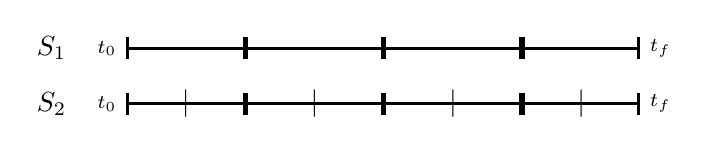
\begin{tikzpicture}%[scale=0.50, every node/.style={scale=0.7}]

	\node at (-12em,0em) (c11) {$S_1$};
	\node at (-12em,-2em) (c11) {$S_2$};
  
	\node at (-10em,0em) (c11) {\scriptsize $t_0$};
	\node at (-10em,-2em) (c21) {\scriptsize $t_0$};

  \node at (-5em,0em) (c12) {};
	\node at (-5em,-2em) (c22) {};
  
    
  \node at (0em,0em) (c13) {};
	\node at (0em,-2em) (c23) {};
  
  \node at (5em,0em) (c14) {};
	\node at (5em,-2em) (c24) {};

  \node at (10em,0em) (c15) {\scriptsize $t_f$};
	\node at (10em,-2em) (c25) {\scriptsize $t_f$};  
  
  
	\draw[line width=1pt, |-|] (c11) -- (c12.center);
	\draw[line width=1pt, |-|] (c12.center) -- (c13.center);
	\draw[line width=1pt, |-|] (c13.center) -- (c14.center);
	\draw[line width=1pt, |-|] (c14.center) -- (c15);
	\draw[line width=1pt, |-|] (c21) -- node[midway]{$|$} (c22.center);
	\draw[line width=1pt, |-|] (c22.center) -- node[midway]{$|$} (c23.center);
	\draw[line width=1pt, |-|] (c23.center) -- node[midway]{$|$} (c24.center);
	\draw[line width=1pt, |-|] (c24.center) -- node[midway]{$|$}  (c25);

	
  \end{tikzpicture}

\end{frame}

\subsection{Objetivos}

\begin{frame}{Introducción}{Objetivos}

Considerando la motivación y la formulación precedente, queda establecido el siguiente objetivo general de la maestría:
\vspace{1em}

\textit{Desarrollar una estrategia de resolución de problemas complejos formulados mediante el
Método de Descomposición Disjunta de Dominios que permita resolver subproblemas separados con códigos de cálculo específicos,
manteniendo la interacción entre ellos solo mediante condiciones de borde.}

\end{frame}
